\documentclass[12pt,letter]{article}
\usepackage{../downey_format}

% ---------------------------------------------------------------------------
% NOTE: TikZ is required for figures 4.3 and 4.11 (the two new drawn figures).
% If downey_format.sty already loads TikZ, these three lines are harmless
% no-ops and can be deleted.
% ---------------------------------------------------------------------------


% ---------------------------------------------------------------------------
% ENVIRONMENT NOTE: this file uses \begin{review} for the call-out boxes,
% because that is the environment confirmed in Chapter 3. If downey_format.sty
% also defines a `note` environment (the blue box), swap them with a
% find/replace on  review -> note  for boxes 4.1, 4.2 and 4.3 below.
% ---------------------------------------------------------------------------


\begin{document}

	% set the section number, along with figure and equation numbers
	\setcounter{section}{3}
	\setcounter{figure}{0}
	\renewcommand\thefigure{\thesection.\arabic{figure}}


\section{Poles, Zeros, and Stability}
\label{sec:poles_zeros_stability}

Chapter~\ref{sec:transfer_functions} showed that any linear, time-invariant system can be written as a transfer function: a ratio of two polynomials in the complex variable $s$. That result is more powerful than it first appears. Once a system is written in this form, its entire character --- whether it settles or runs away, whether it oscillates or creeps, how quickly it does either --- is fixed by a handful of numbers, and those numbers can be found by factoring a polynomial. No differential equation needs to be solved, and no time response needs to be computed.

Those numbers are the \textbf{poles} and \textbf{zeros} of the system. This chapter defines them, shows what they look like in the complex plane, and establishes the single most important result in classical control: \emph{a system is stable if and only if all of its poles lie in the left half of the complex plane}. Everything in the later chapters --- performance indicators, root locus, stability margins, controller design --- is built on that statement.


\subsection{The \texorpdfstring{$s$}{s}-Plane, Poles, and Zeros}
\label{sec:poles_and_zeros}

Recall from equation~\ref{eq:transfer_function_polynominal_expansion} that the transfer function of a general system is the ratio of two polynomials,
\begin{equation}
	G(s) = H(s) = \frac{X(s)}{F(s)} = \frac{B(s)}{A(s)} = \frac{b_ms^m+b_{m-1}s^{m-1} + \cdots + b_0}{a_ns^n+a_{n-1}s^{n-1} + \cdots + a_0}
	\label{eq:transfer_function_ratio}
\end{equation}
where $B(s)$ carries the input side of the equation of motion and $A(s)$ carries the output side.

The variable $s$ is complex. Writing it in terms of its real and imaginary parts,
\begin{equation}
	s = \sigma + i \omega
	\label{eq:s_definition}
\end{equation}
means that $s$ is not a point on a line but a point on a \emph{plane}, called the $s$-plane. The horizontal axis measures $\sigma$, the real part, and the vertical axis measures $\omega$, the imaginary part. Every point on that plane is a value that can be substituted into equation~\ref{eq:transfer_function_ratio}, and each substitution returns a complex number $G(s)$. Taking the magnitude of that number, $|G(s)|$, and plotting it as a height above the plane produces a surface. \textbf{That surface is the picture of the transfer function.} It is what is being plotted in the three-dimensional figures throughout this chapter, and reading it correctly makes the rest of the chapter straightforward.

Two features of that surface matter, and both come from the fact that equation~\ref{eq:transfer_function_ratio} is a fraction.

\begin{enumerate}
	\item A \textbf{pole} is a value of $s$ that makes the denominator vanish, i.e. a root of $A(s) = 0$. Dividing by zero sends $|G(s)| \rightarrow \infty$, so a pole appears on the surface as a spike shooting upward toward infinity.
	\item A \textbf{zero} is a value of $s$ that makes the numerator vanish, i.e. a root of $B(s) = 0$. There $|G(s)| = 0$, so a zero appears as a point where the surface is pinned down to the floor.
\end{enumerate}

Both are properties of the system alone. They do not depend on what the system is fed --- this is the same point made in section~\ref{sec:transfer_function_steady_state}, where a cosine input and a sine input produced the same $H(s)$.

Because the spike at a pole is infinitely tall and the dimple at a zero is a single point, the full three-dimensional surface is often more detail than is needed. The standard shorthand is the \textbf{pole-zero map}: a flat drawing of the $s$-plane with each pole marked $\times$ and each zero marked $\circ$. Figure~\ref{fig:transfer_function_poles_and_zeros_and_3D_space} shows both representations of the same system side by side.

			\begin{figure}[H]
				\centering
				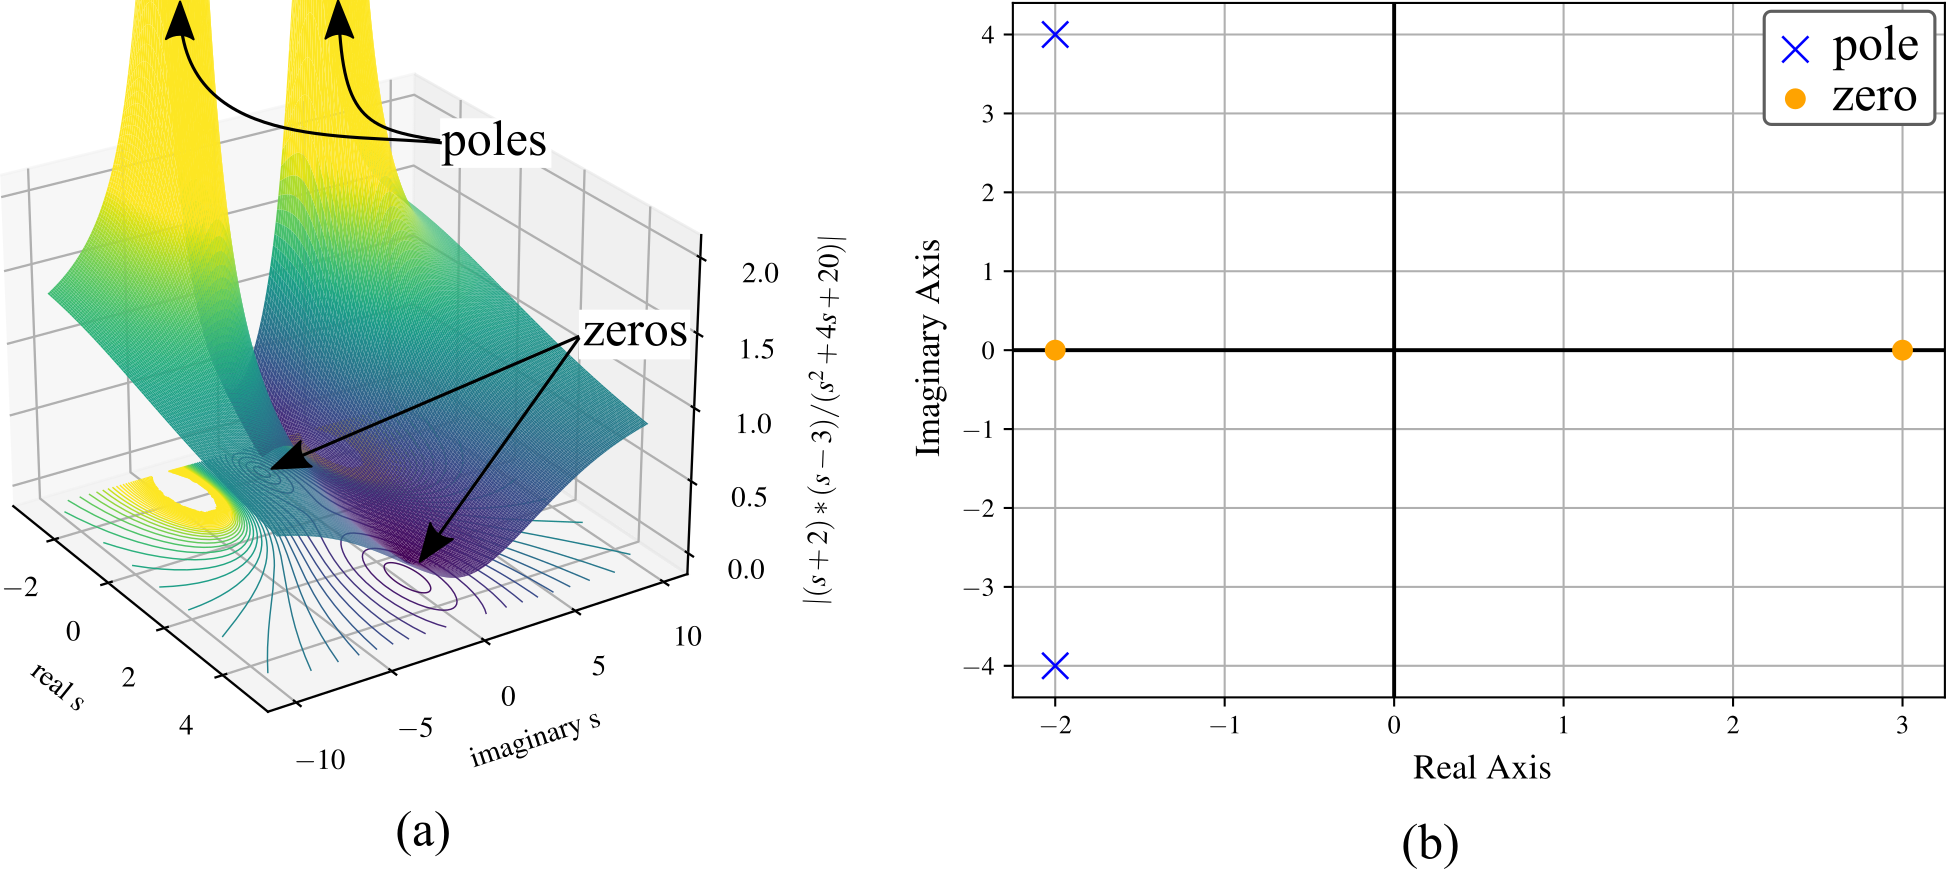
\includegraphics[width=5.0in]{../figures/transfer_function_poles_and_zeros_and_3D_space.png}
				\caption{Poles and zeros of the transfer function $\sfrac{(s+2)(s-3)}{s^2+4s+20}$, showing: (a) the magnitude $|G(s)|$ plotted as a surface over the complex $s$-plane, where poles rise to infinity and zeros are pinned to zero; and (b) the same information as a pole-zero map, with poles marked $\times$ and zeros marked $\circ$.}
				\label{fig:transfer_function_poles_and_zeros_and_3D_space}
			\end{figure}

Finding the poles and zeros of a system requires nothing more than factoring the two polynomials.

\begin{example}
	Find the poles and zeros of the system plotted in figure~\ref{fig:transfer_function_poles_and_zeros_and_3D_space},
	\begin{equation}
		G(s) = \frac{(s+2)(s-3)}{s^2+4s+20}
	\end{equation}

	\noindent \textbf{Solution:} The numerator is already factored, so the zeros can be read directly:
	\begin{equation}
		B(s) = (s+2)(s-3) = 0 \; \; \rightarrow \; \; z_1 = -2, \; \; z_2 = 3
	\end{equation}
	Both zeros are real, so both lie on the horizontal axis of the $s$-plane.

	The denominator requires the quadratic formula:
	\begin{align}
		A(s) &= s^2+4s+20 = 0 \\
		p_{1,2} &= \frac{-4 \pm \sqrt{4^2 - 4(1)(20)}}{2(1)} \nonumber \\
		&= \frac{-4 \pm \sqrt{-64}}{2} \nonumber \\
		&= -2 \pm 4i \nonumber
	\end{align}
	The radicand is negative, so the poles are a complex conjugate pair, $p_{1,2} = -2 \pm 4i$.

	Comparing to figure~\ref{fig:transfer_function_poles_and_zeros_and_3D_space}(b): the two zeros sit on the real axis at $-2$ and $+3$, and the two poles sit at a height of $\pm 4$ above and below the real axis at $-2$. Both poles have a real part of $-2$, which places them in the left half of the plane. Section~\ref{sec:pole_location} shows why that single observation is enough to conclude the system is stable.

	In MATLAB the same result is obtained with \texttt{roots(B)} and \texttt{roots(A)}, or directly from a transfer function object with \texttt{zero(G)} and \texttt{pole(G)}.
\end{example}

Figure~\ref{fig:transfer_function_3D_space_3_examples} plots three more surfaces, chosen to isolate the two features. In (a), $H(s) = s-1$ has a single zero at $s=1$ and no poles at all --- the surface is a bowl that touches zero at that point. In (b), $H(s) = \sfrac{1}{s-1}$ has a single pole at the same location $s = 1$, and the surface spikes to infinity there instead. Comparing (a) and (b) is the cleanest illustration available of the difference between a zero and a pole: same point in the plane, opposite behaviour. In (c), $H(s) = \sfrac{(-20s+20)}{(s+2)}$ has both, a zero at $s=1$ and a pole at $s=-2$.

			\begin{figure}[H]
				\centering
				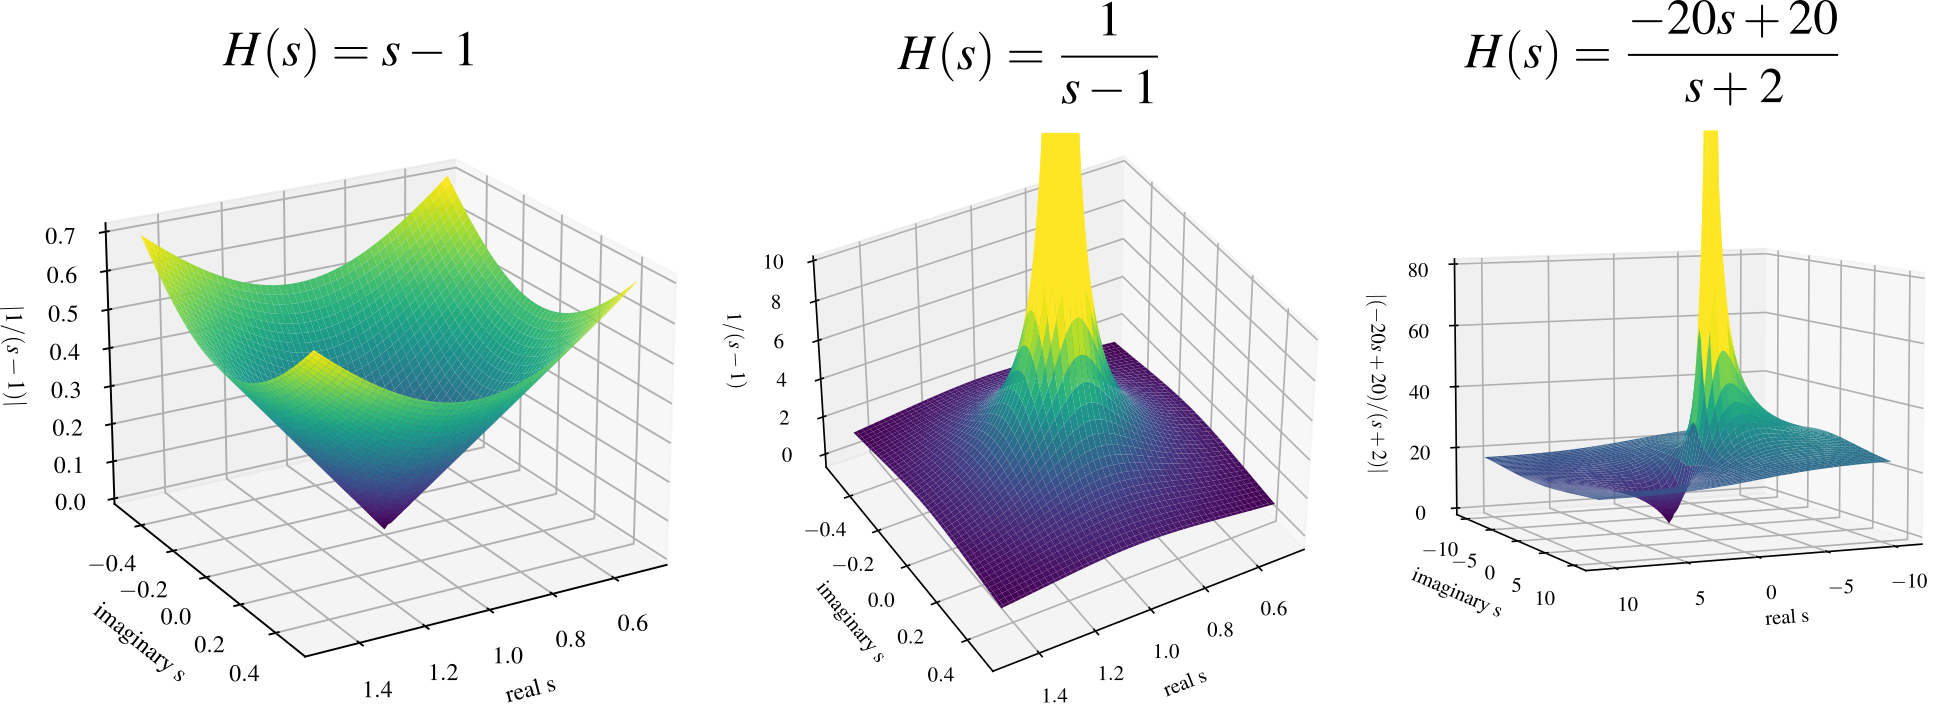
\includegraphics[width=6.5in]{../figures/transfer_function_3D_space_3_examples.png}
				\caption{The magnitude $|H(s)|$ plotted over the complex plane for three transfer functions, isolating the effect of each feature: (a) a single zero at $s=1$; (b) a single pole at the same location $s=1$; and (c) a zero at $s=1$ together with a pole at $s=-2$.}
				\label{fig:transfer_function_3D_space_3_examples}
			\end{figure}

Not every ratio of polynomials describes a system that can be built. The relevant condition is a comparison of the two polynomial orders in equation~\ref{eq:transfer_function_ratio}, $n$ for the denominator and $m$ for the numerator:

\begin{itemize}
	\item \textbf{Proper}: $n \geq m$. There are at least as many poles as zeros. All physically realizable systems are proper.
	\item \textbf{Strictly proper}: $n > m$. There are strictly more poles than zeros. Most mechanical systems fall here.
	\item \textbf{Improper}: $m > n$. More zeros than poles. Such a system would have to differentiate its input more times than it integrates, which requires it to anticipate the future, and it cannot be built.
\end{itemize}

\noindent Case (a) of figure~\ref{fig:transfer_function_3D_space_3_examples} is worth a second look on this point. $H(s) = s-1$ has $m=1$ and $n=0$, making it improper: it is a pure differentiator, useful as a mathematical building block but not realizable on its own as a physical system.

\begin{review}
	\label{sec:characteristic_roots_are_poles}
	\textbf{Characteristic roots and poles are the same numbers}

	The symbol $p$ has appeared before. In chapter~\ref{sec:systems}, solving the equation of motion of the damped oscillator began by assuming a solution of the form $x(t) = Ce^{pt}$, substituting it into the equation of motion, and arriving at the \emph{characteristic equation}
	\begin{equation}
		mp^2 + cp + k = 0
	\end{equation}
	whose roots $p_{1,2}$ governed whether the free response decayed or grew.

	In section~\ref{sec:transfer_function_steady_state} the transfer function of that same oscillator was derived as
	\begin{equation}
		H(s) = \frac{1}{ms^2+cs+k}
	\end{equation}

	These are the same polynomial. The characteristic equation is the denominator of the transfer function, with $p$ renamed $s$. It follows that the characteristic roots of chapter~\ref{sec:systems} \emph{are} the poles of this chapter --- not merely analogous quantities, but the same numbers arrived at by two different routes.

	This is worth stating plainly because it means the stability results developed here are not a new theory. They are the general form of what was already established for first- and second-order systems, extended to systems of any order, and expressed in a way that can be read off a diagram rather than solved for.
\end{review}


\subsection{What Pole Location Tells You}
\label{sec:pole_location}

The claim made in the introduction was that pole locations determine the behaviour of the system. This section establishes why, and it is the conceptual centre of the chapter.

Start from the result of section~\ref{sec:inverse_laplace}. Any output $X(s)$ can be expanded in partial fractions and inverted term by term,
\begin{equation}
	X(s) = \sum_{i=1}^{n} \frac{r_i}{s-p_i} \; \; \; \xrightarrow{\Laplace{\; \; \;}^{-1}} \; \; \; x(t) = \sum_{i=1}^{n} r_i e^{p_i t}
	\label{eq:response_as_sum_of_poles}
\end{equation}
Read equation~\ref{eq:response_as_sum_of_poles} carefully, because it contains the whole argument. \textbf{Every pole of the system contributes exactly one exponential term to the response.} The residues $r_i$ set how strongly each term is excited, but the poles $p_i$ sit in the exponents, and the exponent is what decides whether a term grows or dies.

Now substitute the complex form of the pole, $p = \sigma + i \omega$, into a single term and split it using Euler's formula (review~\ref{sec:Eulers_formula}):
\begin{equation}
	e^{pt} = e^{(\sigma + i \omega)t} = \underbrace{e^{\sigma t}}_\text{envelope} \cdot \underbrace{e^{i \omega t}}_\text{oscillation}
	\label{eq:pole_term_split}
\end{equation}
The term separates cleanly into two factors, and each one is controlled by a different coordinate of the pole:

\begin{itemize}
	\item $e^{i \omega t} = \cos(\omega t) + i \sin(\omega t)$ has a magnitude of exactly $1$ for all time. It never grows and never decays; it only rotates. The \textbf{imaginary part $\omega$ --- the vertical position of the pole --- sets how fast the response oscillates}, and nothing else.
	\item $e^{\sigma t}$ is a real exponential with no oscillation in it at all. It is the envelope inside which the oscillation happens. The \textbf{real part $\sigma$ --- the horizontal position of the pole --- decides whether that envelope shrinks or grows}.
\end{itemize}

That second point is the whole of stability, and it reduces to the sign of $\sigma$:

\begin{itemize}
	\item If $\sigma < 0$, the pole lies in the \textbf{left half-plane}. Then $e^{\sigma t} = e^{-|\sigma| t}$, which decays toward zero. Whatever the term did initially, it dies out. \textbf{Stable.}
	\item If $\sigma > 0$, the pole lies in the \textbf{right half-plane}. Then $e^{\sigma t}$ grows without bound. The term takes over the response and runs away. \textbf{Unstable.}
	\item If $\sigma = 0$, the pole lies exactly \textbf{on the imaginary axis}. Then $e^{\sigma t} = e^0 = 1$, a constant envelope. The term neither decays nor grows, and oscillation continues forever at fixed amplitude. This is the boundary between the two, and it is treated separately in section~\ref{sec:marginal_stability}.
\end{itemize}

\noindent The imaginary axis is therefore the \textbf{stability boundary}: it is the dividing line between poles that die out and poles that blow up. Figure~\ref{fig:pole_location_stability} collects this into a single picture.

\begin{figure}[H]
	\centering
	\begin{tikzpicture}[>=Stealth,scale=1.0]

		% --- shaded half planes -------------------------------------------
		\fill[green!7]  (-5.0,-2.6) rectangle (0,2.6);
		\fill[red!7]    (0,-2.6) rectangle (5.0,2.6);

		% --- axes ---------------------------------------------------------
		\draw[->,thick] (-5.2,0) -- (5.4,0) node[right] {$\sigma = \mathrm{Re}(s)$};
		\draw[->,thick] (0,-2.8) -- (0,2.9) node[above] {$i\omega = \mathrm{Im}(s)$};

		% --- region labels ------------------------------------------------
		\node[align=center,green!45!black] at (-3.4,2.25)
			{\footnotesize \textbf{LEFT half-plane} \\[-1pt] \footnotesize $\sigma<0$ \quad decays \quad \textbf{STABLE}};
		\node[align=center,red!55!black] at (3.4,2.25)
			{\footnotesize \textbf{RIGHT half-plane} \\[-1pt] \footnotesize $\sigma>0$ \quad grows \quad \textbf{UNSTABLE}};
		\node[align=center,rotate=90,gray!60!black] at (-0.75,-1.85) {\scriptsize stability boundary};

		% --- pole markers -------------------------------------------------
		% (1) real, LHP
		\draw[thick] (-3.6,-0.14) -- (-3.4,0.14);  \draw[thick] (-3.6,0.14) -- (-3.4,-0.14);
		\node at (-3.5,-0.45) {\scriptsize \textcircled{\scriptsize 1}};
		% (2) complex pair, LHP
		\draw[thick] (-1.9,1.06) -- (-1.7,1.34);   \draw[thick] (-1.9,1.34) -- (-1.7,1.06);
		\draw[thick] (-1.9,-1.34) -- (-1.7,-1.06); \draw[thick] (-1.9,-1.06) -- (-1.7,-1.34);
		\node at (-2.15,1.55) {\scriptsize \textcircled{\scriptsize 2}};
		% (3) on the axis
		\draw[thick] (-0.1,1.66) -- (0.1,1.94);    \draw[thick] (-0.1,1.94) -- (0.1,1.66);
		\draw[thick] (-0.1,-1.94) -- (0.1,-1.66);  \draw[thick] (-0.1,-1.66) -- (0.1,-1.94);
		\node at (0.42,1.95) {\scriptsize \textcircled{\scriptsize 3}};
		% (4) complex pair, RHP
		\draw[thick] (1.7,1.06) -- (1.9,1.34);     \draw[thick] (1.7,1.34) -- (1.9,1.06);
		\draw[thick] (1.7,-1.34) -- (1.9,-1.06);   \draw[thick] (1.7,-1.06) -- (1.9,-1.34);
		\node at (2.15,1.55) {\scriptsize \textcircled{\scriptsize 4}};
		% (5) real, RHP
		\draw[thick] (3.4,-0.14) -- (3.6,0.14);    \draw[thick] (3.4,0.14) -- (3.6,-0.14);
		\node at (3.5,-0.45) {\scriptsize \textcircled{\scriptsize 5}};

		% ==================================================================
		% time response strip
		% ==================================================================
		\begin{scope}[yshift=-4.9cm,xshift=-4.6cm]

		\foreach \k/\lab in {0/1,1/2,2/3,3/4,4/5}{
			\begin{scope}[xshift=\k*2.35cm]
				\draw[->] (0,0) -- (1.75,0) node[right] {\tiny $t$};
				\draw[->] (0,-0.85) -- (0,0.95);
				\node at (0.85,-1.15) {\scriptsize \textcircled{\scriptsize \lab}};
			\end{scope}
		}

		% (1) decaying exponential
		\draw[thick,green!45!black,domain=0:1.6,samples=60]
			plot (\x,{0.8*exp(-1.7*\x)});
		% (2) decaying oscillation
		\begin{scope}[xshift=2.35cm]
			\draw[thick,green!45!black,domain=0:1.6,samples=140]
				plot (\x,{0.8*exp(-1.1*\x)*sin(360*\x/0.75)});
			\draw[dashed,gray,domain=0:1.6,samples=60] plot (\x,{0.8*exp(-1.1*\x)});
		\end{scope}
		% (3) sustained oscillation
		\begin{scope}[xshift=4.70cm]
			\draw[thick,orange!80!black,domain=0:1.6,samples=140]
				plot (\x,{0.62*sin(360*\x/0.75)});
		\end{scope}
		% (4) growing oscillation
		\begin{scope}[xshift=7.05cm]
			\draw[thick,red!70!black,domain=0:1.6,samples=140]
				plot (\x,{0.11*exp(1.2*\x)*sin(360*\x/0.75)});
			\draw[dashed,gray,domain=0:1.6,samples=60] plot (\x,{0.11*exp(1.2*\x)});
		\end{scope}
		% (5) growing exponential
		\begin{scope}[xshift=9.40cm]
			\draw[thick,red!70!black,domain=0:1.6,samples=60]
				plot (\x,{0.12*exp(1.3*\x)});
		\end{scope}

		\end{scope}
	\end{tikzpicture}
	\caption{Pole location in the complex plane and the corresponding contribution to the time response. Moving left to right across the plane changes the response from decaying to growing, while moving away from the real axis adds oscillation. Poles \textcircled{\scriptsize 1} and \textcircled{\scriptsize 2} lie in the left half-plane and decay; pole pair \textcircled{\scriptsize 3} lies on the stability boundary and oscillates forever; poles \textcircled{\scriptsize 4} and \textcircled{\scriptsize 5} lie in the right half-plane and grow without bound.}
	\label{fig:pole_location_stability}
\end{figure}

Reading figure~\ref{fig:pole_location_stability} across the horizontal direction gives the growth-or-decay behaviour, and reading it in the vertical direction gives the oscillation. A pole far to the left decays quickly; a pole just barely to the left decays slowly; a pole just barely to the right grows slowly but grows nonetheless. There is no partial credit at the boundary --- a pole with $\sigma = -0.001$ is stable and a pole with $\sigma = +0.001$ is not, even though the two responses look nearly identical for the first several seconds.

Physically, the sign of $\sigma$ answers whether the system removes energy from itself or supplies energy to itself. A left-half-plane pole corresponds to a mechanism that dissipates --- damping, friction, electrical resistance --- so a disturbance is bled away and the system returns to where it started. A right-half-plane pole corresponds to a mechanism that feeds energy in faster than it is removed, so a disturbance is amplified. This is not an exotic condition. Aeroelastic flutter, thermal runaway, and a feedback controller with too much gain are all cases of an engineered system placing one of its own poles in the right half-plane.

\begin{review}
	\label{sec:rhp_pole_already_seen}
	\textbf{A right-half-plane pole has already appeared}

	Section~\ref{sec:laplace_exponential} derived the transform pair
	\begin{equation}
		f(t) = e^{p_0 t} \; \; \; \longleftrightarrow \; \; \; F(s) = \frac{1}{s-p_0}
	\end{equation}
	and noted that $p_0$ is a pole because $F(s) \rightarrow \infty$ as $s \rightarrow p_0$.

	Figure~\ref{fig:S_space_exp_pt} plotted that pair for the specific value $p_0 = 5$. Since $p_0$ is real and positive, it sits at $\sigma = +5$ on the horizontal axis --- in the right half-plane. Looking back at the time-domain plot in figure~\ref{fig:S_space_exp_pt}(a) confirms the prediction: the response runs off the top of the axes.

	That figure was presented as a transform pair, but it was also the first unstable system in this text.
\end{review}

One consequence of equation~\ref{eq:response_as_sum_of_poles} deserves emphasis, because the chapter title mentions zeros and they have gone quiet since section~\ref{sec:poles_and_zeros}. \textbf{Zeros do not affect stability.} Only the poles appear in the exponents, so only the poles decide growth or decay. Zeros influence the residues $r_i$, which is to say they change how strongly each mode is excited and therefore the shape, overshoot, and phase of the response. A zero can make a response ugly. It cannot make it unstable. Every stability criterion in this chapter looks only at $A(s)$.


\subsection{Stability of Response}
\label{sec:stability_of_response}

With the mechanism established, the definitions can be stated:

\begin{center}
	\textit{A system is stable if any bounded input excitation produces a bounded output response.}
\end{center}

\begin{figure}[H]
	\centering
	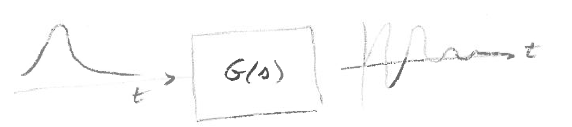
\includegraphics[width=5.5in]{../figures/stable_system_block_diagram}
	\caption{A bounded input applied to a stable system produces a bounded output.}
	\label{fig:stable_system_block_diagram}
\end{figure}

\begin{center}
	\textit{A response is stable if it remains bounded as $t \rightarrow \infty$.}
\end{center}

\noindent The word \emph{bounded} is doing the work in both statements. It does not mean the response is small, settles quickly, or behaves nicely --- only that some finite ceiling exists that it never exceeds. Figure~\ref{fig:stable_responses} shows bounded responses for first- and second-order systems.

\begin{figure}[H]
	\centering
	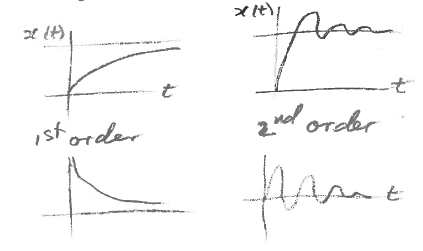
\includegraphics[width=4.5in]{../figures/stable_responses}
	\caption{Bounded responses for first-order and second-order systems. In each case the response settles to a finite value as $t \rightarrow \infty$.}
	\label{fig:stable_responses}
\end{figure}

The following three subsections apply the result of section~\ref{sec:pole_location} to systems of increasing order. The pattern is the same in all three, which is the point: the argument does not get harder as systems get more complicated.

\subsubsection{Stability of 1\textsuperscript{st}-Order Responses}
\label{sec:stability_first_order}

A first-order system has a single pole, so equation~\ref{eq:response_as_sum_of_poles} has a single term:
\begin{equation}
	X(s) = \frac{K}{s-p}
	\; \; \; \xrightarrow{\Laplace{\; \; \;}^{-1}} \; \; \;
	x(t) = K e^{p t}
	\label{eq:first_order_pole_response}
\end{equation}
where $p$ is the pole of $X(s)$. A single real pole has no imaginary part, so there is no oscillation and the entire behaviour is the envelope $e^{pt}$. Stability is dictated by the sign of $p$, i.e. its location along the real axis:

\begin{itemize}
	\item $p < 0$ (left half-plane): the response decays as $e^{-|p|t}$. If a disturbing force is applied, the system returns to its initial state. \textbf{Stable.}
	\item $p = 0$ (origin): the response is $Ke^0 = K$, a constant. The system holds wherever it is put and neither returns nor runs away. \textbf{Marginal.}
	\item $p > 0$ (right half-plane): the response grows as $e^{pt}$ without bound. \textbf{Unstable.}
\end{itemize}

\noindent These three cases are shown in figure~\ref{fig:system_stability_first_order}, with the pole location in the complex plane drawn beneath each response.

\begin{figure}[H]
	\centering
	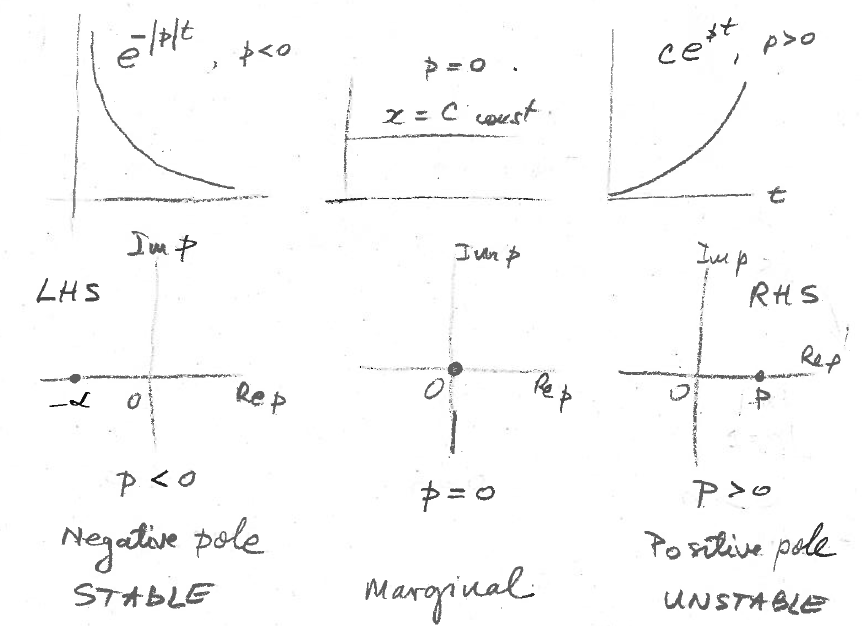
\includegraphics[width=4.5in]{../figures/system_stability_first_order}
	\caption{The three possible behaviours of a single real pole, showing the time response above and the corresponding pole location in the complex plane below: a negative pole in the left half-plane decays and is stable; a pole at the origin is marginal; and a positive pole in the right half-plane grows and is unstable.}
	\label{fig:system_stability_first_order}
\end{figure}

\noindent Recall from section~\ref{sec:first_order_systems} that the first-order system was written in standard form with a time constant $T$, giving a pole at $p = -\sfrac{1}{T}$. A positive time constant therefore places the pole in the left half-plane automatically, which is why every physical first-order system built from a spring and damper is stable.

\subsubsection{Stability of 2\textsuperscript{nd}-Order Responses}
\label{sec:stability_second_order}

A second-order system has two poles, and equation~\ref{eq:response_as_sum_of_poles} becomes a sum of two terms. Written with its zero shown explicitly,
\begin{equation}
	X(s) = \frac{k(s-z_1)}{(s-p_1)(s-p_2)}
	\label{eq:second_order_pole_zero_form}
\end{equation}
The two poles are either both real, or a complex conjugate pair --- they cannot be complex independently, because $A(s)$ has real coefficients. This gives seven distinct arrangements, catalogued in figure~\ref{fig:2nd_order_poles}:

\begin{enumerate}
	\item $p_1, p_2 < 0$, two distinct negative real poles in the left half-plane. Both terms decay with no oscillation: monotonic decay, \textbf{stable}.
	\item $p_1 = p_2 < 0$, a negative real double pole in the left half-plane. Still monotonic decay, \textbf{stable}. This is the critically damped case and is the fastest non-oscillating response available.
	\item $p_{1,2} = \sigma \pm i\omega$ with $\sigma < 0$, a complex pair in the left half-plane. The envelope decays while the response oscillates inside it: damped oscillation, \textbf{stable}.
	\item $p_{1,2} = \pm i\omega$ with $\sigma = 0$, a purely imaginary pair on the axis. Constant envelope, so oscillation continues forever: \textbf{at the limit of stability}.
	\item $p_{1,2} = \sigma \pm i\omega$ with $\sigma > 0$, a complex pair in the right half-plane. Growing envelope with oscillation inside it: \textbf{unstable}.
	\item $p_1 = p_2 > 0$, a positive real double pole in the right half-plane. Monotonic growth, \textbf{unstable}.
	\item $p_1, p_2 > 0$, two distinct positive real poles in the right half-plane. Monotonic growth, \textbf{unstable}.
\end{enumerate}

\begin{figure}[H]
	\centering
	
\includegraphics[width=4.5in]{../figures/2nd_order_poles}
	\caption{The seven possible pole arrangements for a second-order system, with the pole location in the complex plane and the resulting time response. Cases 1 through 3 are stable, case 4 sits at the limit of stability, and cases 5 through 7 are unstable. Cases 3 through 5 oscillate; the remainder are monotonic.}
	\label{fig:2nd_order_poles}
\end{figure}

Reading down the figure, the seven cases divide along the two axes established in section~\ref{sec:pole_location}. Cases 1, 2, 6 and 7 have no imaginary part and so do not oscillate. Cases 3, 4 and 5 do. Independently of that, cases 1 through 3 sit in the left half-plane and decay, case 4 sits on the boundary, and cases 5 through 7 sit in the right half-plane and grow.

Note also what is \emph{not} in the list: the zero $z_1$ from equation~\ref{eq:second_order_pole_zero_form} never appears. It affects the residues and therefore the shape of each response, but it plays no part in the classification.

\begin{review}
	\label{sec:damping_ratio_and_poles}
	\textbf{Where the damping ratio sits in the plane}

	Section~\ref{sec:spring_mass_damper} found the poles of the damped oscillator to be
	\begin{equation}
		p_{1,2} = -\zeta \omega_n \pm i \omega_d
	\end{equation}
	Comparing this to $p = \sigma + i\omega$ identifies the two coordinates directly:
	\begin{equation}
		\sigma = -\zeta \omega_n \; \; \; \text{and} \; \; \; \omega = \omega_d
	\end{equation}

	The real part is set entirely by the damping. Positive damping $\zeta > 0$ makes $\sigma$ negative and places the poles in the left half-plane, which is why adding a damper stabilises a system. Zero damping puts them on the imaginary axis at $p_{1,2} = \pm i\omega_n$, which is case 4 above and explains why an undamped oscillator rings forever. Negative damping --- a system that extracts energy from its environment rather than dissipating it --- moves the poles into the right half-plane.

	Cases 1 through 3 of figure~\ref{fig:2nd_order_poles} are therefore the overdamped, critically damped, and underdamped responses of section~\ref{sec:spring_mass_damper}, seen from the $s$-plane instead of the time domain.
\end{review}

\subsubsection{Stability of Higher-order Responses}
\label{sec:stability_higher_order}

Nothing new is required for systems of arbitrary order. Starting from the general expression for the output of a system,
\begin{equation}
	X(s) = \frac{B(s)}{A(s)} = \frac{b_ms^m+b_{m-1}s^{m-1} + \cdots + b_0}{a_ns^n+a_{n-1}s^{n-1} + \cdots + a_0}
\end{equation}
partial fraction expansion results in
\begin{equation}
	X(s) = \frac{r_1}{s-p_1} + \frac{r_2}{s-p_2} + \cdots + \frac{r_n}{s-p_n}
\end{equation}
where $p_1, \; p_2, \; \cdots \; p_n$ are the poles of the system (i.e. roots of $A(s)=0$) and $r_1,\; r_2,\; \cdots \; r_n$ are the residues of the system. Note that the poles can either be real or complex. Again, MATLAB can be used to solve for the roots, poles, and gains of the system using \texttt{[r,p,k]=residue(B,A)}.

The real poles can be
\begin{itemize}
	\item single pole: $\frac{r}{s-p} \xrightarrow{\Laplace{\; \; \;}^{-1}} re^{pt}$
	\item double poles: $\frac{r}{(s-p)^2} \xrightarrow{\Laplace{\; \; \;}^{-1}} rte^{pt}$
	\item multiple poles: $\frac{r}{(s-p)^j} \xrightarrow{\Laplace{\; \; \;}^{-1}} \frac{1}{(j-1)!}t^{j-1}e^{pt}$
\end{itemize}
where stable and unstable responses are shown in figure~\ref{fig:stability_higher_order_systems_real_poles}. Repeating a pole introduces a polynomial factor $t^{j-1}$ alongside the exponential, but it does not change the conclusion: for $p<0$ the exponential decays faster than any power of $t$ grows, so the product still decays.

\begin{figure}[H]
	\centering
	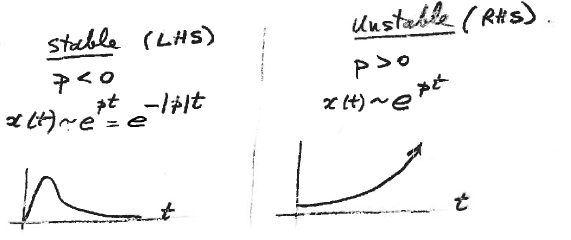
\includegraphics[width=4.5in]{../figures/stability_higher_order_systems_real_poles}
	\caption{Behaviour of a single real-pole term from the partial fraction expansion. A pole in the left half-plane ($p<0$) produces a decaying exponential, while a pole in the right half-plane ($p>0$) produces a growing one.}
	\label{fig:stability_higher_order_systems_real_poles}
\end{figure}

The complex poles are always in conjugate pairs, and are governed by $p_{1,2}=\sigma \pm i \omega$ where
\begin{itemize}
	\item first pole: $\frac{r}{s-p_1} = \frac{r}{s-(\sigma + i \omega)} \xrightarrow{\Laplace{\; \; \;}^{-1}} re^{(\sigma + i \omega)t} = re^{\sigma t} e^{i \omega t}$
	\item second pole: $\frac{\bar{r}}{s-p_2} = \frac{\bar{r}}{s-(\sigma - i \omega)} \xrightarrow{\Laplace{\; \; \;}^{-1}} \bar{r}e^{(\sigma - i \omega)t} = \bar{r}e^{\sigma t} e^{-i \omega t}$
\end{itemize}
Because $A(s)$ has real coefficients, the residues of a conjugate pole pair are themselves conjugates, $r_2 = \bar{r}_1$. The imaginary parts of the two terms therefore cancel when they are added, and applying Euler's formula leaves a real result:
\begin{equation}
	x(t) = re^{(\sigma + i \omega)t} + \bar{r}e^{(\sigma - i \omega)t} = C e^{\sigma t} \sin(\omega t + \phi)
	\label{eq:complex_pair_response}
\end{equation}
where the amplitude $C$ and phase $\phi$ are set by the residues. Equation~\ref{eq:complex_pair_response} is the same envelope-times-oscillation structure as equation~\ref{eq:pole_term_split}: the pair contributes a sinusoid at frequency $\omega$ contained inside an envelope $e^{\sigma t}$, and the sign of $\sigma$ decides everything. Stable and unstable cases are shown in figure~\ref{fig:stability_higher_order_systems_complex_poles}.

\begin{figure}[H]
	\centering
	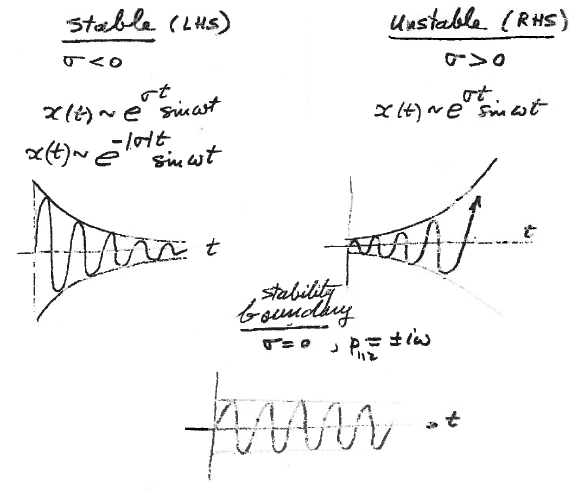
\includegraphics[width=4.5in]{../figures/stability_higher_order_systems_complex_poles}
	\caption{Behaviour of a complex conjugate pole pair. A pair in the left half-plane ($\sigma<0$) oscillates inside a decaying envelope, while a pair in the right half-plane ($\sigma>0$) oscillates inside a growing one. The stability boundary is $\sigma = 0$, where the envelope is constant.}
	\label{fig:stability_higher_order_systems_complex_poles}
\end{figure}

Since the response is the sum of all these terms, and since a sum runs away if any one of its terms runs away, a single pole in the right half-plane is enough to make the entire system unstable no matter how well behaved the remaining poles are. This is what makes the criterion of the next section both simple and strict.


\subsection{Absolute Stability}
\label{sec:absolute_stability}

\begin{center}
	\textit{A necessary and sufficient condition for a system to be stable is that all of its poles are placed in the left hand side of the complex plane.}
\end{center}

\begin{figure}[H]
	\centering
	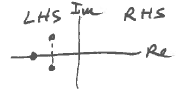
\includegraphics[width=2.5in]{../figures/stable_system_complex_plane_simple}
	\caption{Absolute stability requires every pole to lie strictly within the left half of the complex plane.}
	\label{fig:stable_system_complex_plane_simple}
\end{figure}

The phrase \emph{necessary and sufficient} is worth unpacking, since it is a strong claim in both directions. Necessary means there is no stable system with a right-half-plane pole. Sufficient means that once all poles are confirmed to be in the left half-plane, nothing further needs to be checked.

Three practical consequences follow:

\begin{itemize}
	\item \textbf{Absolute stability is binary.} A system either is or is not stable. There are no degrees, which is precisely why section~\ref{sec:relative_stability} is needed.
	\item \textbf{It does not depend on the input.} The poles come from $A(s)$, which describes the system, not $F(s)$, which describes what the system is fed. A stable system is stable for every bounded input.
	\item \textbf{It does not require solving anything.} There is no need to compute a time response, or even to perform the partial fraction expansion. Factoring $A(s)$ and inspecting the signs of the real parts is sufficient. In MATLAB this is \texttt{roots(A)} or \texttt{pole(G)}.
\end{itemize}

A useful quick check exists before any factoring is attempted. If a polynomial has all its roots in the left half-plane, then all coefficients of $A(s)$ must be present and must share the same sign. Consequently:

\begin{center}
	\textit{If any coefficient of $A(s)$ is zero or differs in sign from the others, the system is unstable.}
\end{center}

\noindent This test is necessary but \emph{not} sufficient --- passing it does not prove stability, it only fails to disprove it. It is nonetheless valuable, because it can rule out a candidate design by inspection. A systematic version of this idea, which extracts a full answer from the coefficients without factoring at all, is developed as the Routh-Hurwitz criterion in section~\ref{sec:stability_criteria}.


\subsection{Marginal Stability}
\label{sec:marginal_stability}

If the poles are purely imaginary (i.e. placed on the imaginary axis) then the system has \textbf{marginal stability}. This is case 4 of figure~\ref{fig:2nd_order_poles}: with $\sigma = 0$ the envelope $e^{\sigma t}$ is constant, so the response neither decays nor grows but oscillates forever at whatever amplitude it was given.

Whether such a system counts as stable depends on what it is fed:
\begin{itemize}
	\item bounded impulse response, the system is stable
	\item unbounded impulse response, or other inputs, the system is not stable.
\end{itemize}

\noindent The reason for this split is worth spelling out, because the two bullets appear to contradict each other. An undamped spring-mass oscillator struck once by a hammer rings at $\omega_n$ forever without growing --- that response is bounded, and by the definition in section~\ref{sec:stability_of_response} it qualifies as stable. But drive that same oscillator with a sinusoid at exactly $\omega_n$ and the amplitude climbs without limit. This is resonance, and the input driving it is perfectly bounded.

Since stability requires a bounded output for \emph{every} bounded input, and a bounded input exists that produces an unbounded output, a marginally stable system is not stable. Marginal stability is the boundary case, not a mild form of stability, and the terminology is easy to misread on that point.

Two further cases sit on the imaginary axis and are worth distinguishing:
\begin{itemize}
	\item A single pole at the \textbf{origin}, $p = 0$, is the case $\sigma = 0$ with $\omega = 0$. There is no oscillation, only a constant. This is a pure integrator, and it is why a system with a free rigid-body mode drifts rather than returning.
	\item \textbf{Repeated} poles on the imaginary axis are genuinely unstable, not marginal. From section~\ref{sec:stability_higher_order}, a double pole contributes $te^{pt}$, and with $\sigma = 0$ that reduces to $t\sin(\omega t)$ --- an oscillation whose amplitude grows linearly with time even under an impulse.
\end{itemize}

\noindent The marginal case therefore requires the imaginary-axis poles to be simple, with all remaining poles strictly in the left half-plane.


\subsection{Dominant Poles}
\label{sec:dominant_poles}

Section~\ref{sec:absolute_stability} answers whether a response dies out. It says nothing about how long that takes, or what the response looks like along the way. For a system with many poles, equation~\ref{eq:response_as_sum_of_poles} contains many terms decaying at many different rates, and in practice a small number of them account for nearly all of the observed behaviour. Those are the \textbf{dominant poles}.

Given
\begin{equation}
	X(s) = \frac{B(s)}{A(s)} = \frac{r_1}{s-p_1} + \frac{r_2}{s-p_2} + \cdots + \frac{r_k}{s-p_k} + \cdots
\end{equation}
where $p_k$ is either a complex number ($p_k \in \mathbb{C}$) in a conjugate pair
\begin{equation}
	p_k = \sigma_k \pm i \omega_k
\end{equation}
or a real number ($p_k \in \mathbb{R}$)
\begin{equation}
	p_k = \sigma_k
\end{equation}
the inverse Laplace transform gives the time series response
\begin{equation}
	x(t) = r_1 e^{p_1 t} + r_2 e^{p_2 t} + \cdots + r_k e^{p_k t} + \cdots
\end{equation}
For controls, we are interested in the long term behaviour of $x(t)$. Every term in the expansion has the form
\begin{equation}
	r_k e^{p_k t} = r_k e^{\sigma_k t} \cdot e^{i \omega_k t}
\end{equation}
where $r_k e^{\sigma_k t}$ is the exponential envelope and $e^{i \omega_k t}$ is the harmonic oscillation. If the system is unstable --- if any $\sigma_k > 0$ --- then that term grows without bound and swamps everything else, which is the situation already settled in section~\ref{sec:absolute_stability}. The interesting case is a stable system, where all $\sigma_k \leq 0$ and every term is decaying or steady. Two situations arise.

\vspace{1ex}
\noindent \textbf{Case A --- Dominant poles on the imaginary axis.} If terms with $\sigma_k = 0$ exist, these will maintain oscillations as the rest of the poles die out. The poles placed on the imaginary axis, if they exist, are therefore the dominant poles. After the transient has passed, the response is whatever those poles are doing, as shown in figure~\ref{fig:dominant_poles_imaginary_axis}.

\begin{figure}[H]
	\centering
	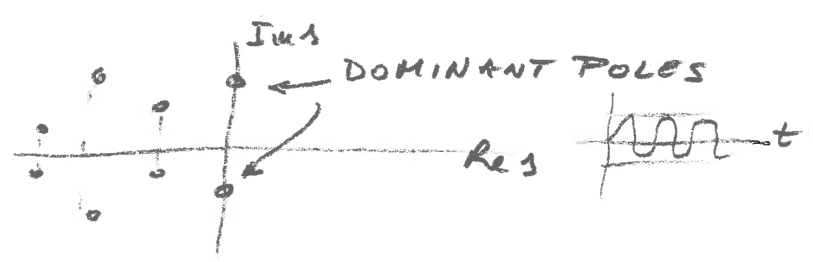
\includegraphics[width=0.8\textwidth]{../figures/dominant_poles_B1.png}
	\caption{System with dominant poles on the imaginary axis. The remaining poles decay away, leaving the sustained oscillation of the imaginary-axis pair as the long-term response.}
	\label{fig:dominant_poles_imaginary_axis}
\end{figure}

\noindent \textbf{Case B --- Dominant poles to the left of the imaginary axis.} If terms with $\sigma_k = 0$ do not exist, then the dominant poles are the poles closest to the imaginary axis, because they take the longest to die out, having small $\sigma_k$ values. Every other term has a more negative $\sigma_k$ and so vanishes sooner, leaving the slowest pair to govern the tail of the response. This is shown in figure~\ref{fig:dominant_poles_left_of_imaginary_axis}.

\begin{figure}[H]
	\centering
	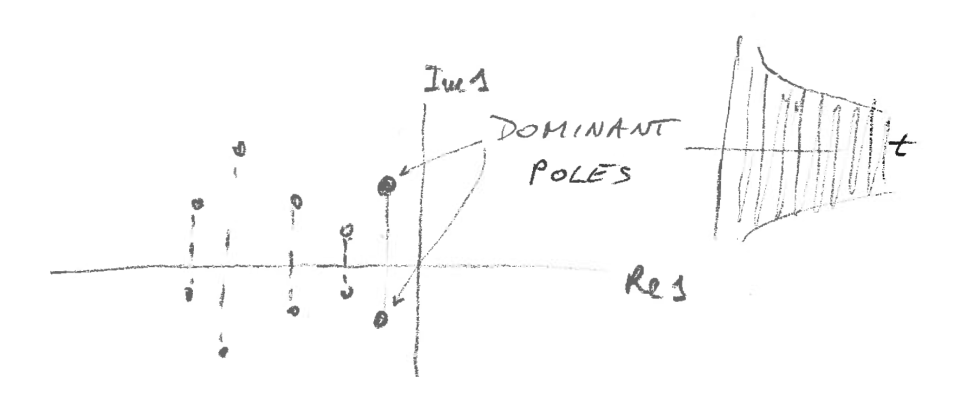
\includegraphics[width=0.8\textwidth]{../figures/dominant_poles_B2.png}
	\caption{System with dominant poles to the left of the imaginary axis. The poles nearest the axis decay most slowly and therefore dictate the long-term response.}
	\label{fig:dominant_poles_left_of_imaginary_axis}
\end{figure}

The practical value of this idea is approximation. A high-order system whose dominant poles are a single complex pair can be analysed as though it were second-order, using that pair alone. The remaining poles contribute only to the first moments of the response. This approximation is what makes the second-order performance indicators of chapter~\ref{sec:performance_indicators} applicable to systems that are not actually second-order, and it is used without further comment throughout the rest of this text.


\subsection{Relative Stability}
\label{sec:relative_stability}

Would a stable system still be stable if its parameters are slightly changed? What margin of safety is there?

These questions are not answered by absolute stability, which returns only yes or no. A system whose dominant pole sits at $\sigma = -0.01$ and one whose dominant pole sits at $\sigma = -10$ are both stable, and the criterion of section~\ref{sec:absolute_stability} cannot distinguish them. Yet the first takes roughly a thousand times longer to settle, and a small change in a physical parameter could push it across the axis. \textbf{Relative stability} is the study of how much margin exists.

The geometry of the pole location supplies the answer, and figure~\ref{fig:relative_stability_geometry} collects the relevant quantities for a complex conjugate pair.

\begin{figure}[H]
	\centering
	\begin{tikzpicture}[>=Stealth,scale=1.0]

		% --- shaded half planes -------------------------------------------
		\fill[green!7] (-4.9,-3.3) rectangle (0,3.3);
		\fill[red!7]   (0,-3.3) rectangle (1.7,3.3);

		% --- axes ---------------------------------------------------------
		\draw[->,thick] (-5.1,0) -- (1.9,0) node[right] {$\sigma$};
		\draw[->,thick] (0,-3.5) -- (0,3.6) node[above] {$i\omega$};
		\node[red!55!black]   at (0.85,-3.05) {\footnotesize \textbf{unstable}};
		\node[green!45!black] at (-4.15,-3.05) {\footnotesize \textbf{stable}};

		% --- the well damped pole pair -------------------------------------
		\coordinate (P)  at (-2.7,2.15);
		\coordinate (Pc) at (-2.7,-2.15);

		\draw[dashed,gray] (P) -- (0,2.15);
		\draw[dashed,gray] (P) -- (-2.7,0);
		\draw[thick,blue!60!black] (0,0) -- (P);
		\draw[thick,blue!60!black] (0,0) -- (Pc);

		% angle theta
		\draw[blue!60!black] (-1.15,0) arc (180:141.5:1.15);
		\node[blue!60!black] at (-1.42,0.42) {\footnotesize $\theta$};

		% pole crosses
		\draw[very thick] ($(P)+(-0.13,-0.13)$) -- ($(P)+(0.13,0.13)$);
		\draw[very thick] ($(P)+(-0.13,0.13)$) -- ($(P)+(0.13,-0.13)$);
		\draw[very thick] ($(Pc)+(-0.13,-0.13)$) -- ($(Pc)+(0.13,0.13)$);
		\draw[very thick] ($(Pc)+(-0.13,0.13)$) -- ($(Pc)+(0.13,-0.13)$);

		% labels
		\node[above] at (-1.55,2.18) {\footnotesize $|\sigma| = \zeta \omega_n$};
		\node[left]  at (-2.78,1.05) {\footnotesize $\omega_d$};
		\node[blue!60!black] at (-0.92,1.28) {\footnotesize $\omega_n$};

		% --- the lightly damped pole pair ----------------------------------
		\coordinate (Q)  at (-0.45,2.85);
		\coordinate (Qc) at (-0.45,-2.85);
		\draw[very thick,gray] ($(Q)+(-0.13,-0.13)$) -- ($(Q)+(0.13,0.13)$);
		\draw[very thick,gray] ($(Q)+(-0.13,0.13)$) -- ($(Q)+(0.13,-0.13)$);
		\draw[very thick,gray] ($(Qc)+(-0.13,-0.13)$) -- ($(Qc)+(0.13,0.13)$);
		\draw[very thick,gray] ($(Qc)+(-0.13,0.13)$) -- ($(Qc)+(0.13,-0.13)$);
		\node[gray!60!black,align=center,anchor=west] at (0.35,3.05)
			{\footnotesize small margin \\[-2pt] \footnotesize (lightly damped)};
		\draw[->,gray!60!black] (0.30,2.95) -- (-0.28,2.87);

	\end{tikzpicture}
	\caption{Geometry of a complex conjugate pole pair in the $s$-plane. The horizontal distance from the imaginary axis, $|\sigma| = \zeta \omega_n$, sets the decay rate; the vertical distance $\omega_d$ sets the oscillation frequency; the radial distance is the natural frequency $\omega_n$; and the angle from the negative real axis satisfies $\cos \theta = \zeta$. The grey pair sits close to the axis and therefore has little stability margin.}
	\label{fig:relative_stability_geometry}
\end{figure}

Reading the figure gives three distinct measures of margin:

\begin{itemize}
	\item \textbf{Distance from the imaginary axis}, $|\sigma| = \zeta \omega_n$. This is the decay rate. A pole far from the axis settles quickly and can tolerate a large parameter change before crossing; a pole near the axis cannot. This distance is what section~\ref{sec:dominant_poles} identified as selecting the dominant poles, so relative stability is normally assessed on the dominant pair alone.
	\item \textbf{Angle from the negative real axis}, where $\cos \theta = \zeta$. Poles near the real axis are well damped and settle without much overshoot; poles near the imaginary axis have $\zeta$ approaching zero and ring badly. The angle is therefore a direct read of the damping ratio off the diagram.
	\item \textbf{Radial distance from the origin}, $\omega_n$. This sets the overall speed of the response without changing its shape --- moving a pole pair radially outward makes everything happen faster at the same damping ratio.
\end{itemize}

Parameter variation is what makes this matter in practice. Stiffness changes with temperature, damping changes as seals wear, mass changes as fuel burns off, and every manufactured component carries a tolerance. Each of these moves the poles. A design whose dominant poles sit comfortably inside the left half-plane absorbs that movement; a design whose poles sit just inside the boundary may not survive a cold morning.

Two later chapters make this quantitative rather than qualitative. The \textbf{root locus} of section~\ref{sec:root_locus} traces the paths the poles follow as a controller gain is varied, showing directly how much gain a design can absorb before a pole crosses into the right half-plane. The \textbf{gain and phase margins} of section~\ref{sec:stability_margins} measure the same distance-from-instability in the frequency domain, where it can be read from experimental data on a system whose poles were never known in the first place.

\end{document}
